\documentclass[a4paper, 14pt]{extarticle}

\usepackage{../generalPreamble}
\usepackage{../reportFormat}
\setcounter{MaxMatrixCols}{20}

\newcommand\sbullet[1][.5]{\mathbin{\vcenter{\hbox{\scalebox{#1}{$\bullet$}}}}}

\begin{document}

\begin{titlepage}
    \centering
    {\bfseries
        \uppercase{
            Минобрнауки России \\
            Санкт-Петербургский государственный \\
            Электротехнический университет \\
            \enquote{ЛЭТИ} им. В.И.Ульянова (Ленина)\\
        }
        Кафедра ИБ

        \vspace{\fill}
        \uppercase{Лабораторная работа №5} \\
        по дисциплине \enquote{Криптография и защита информации} \\
        Тема: Изучение шифра AES
    }

    \vspace{\fill}
    \begin{tabularx}{0.8\textwidth}{l X c r}
        Студент гр. 6304 & & \underline{\hspace{3cm}} & Корытов П.В.\\
        Преподаватель & & \underline{\hspace{3cm}} & Племянников А.К.
    \end{tabularx}

    \vspace{1cm}
    Санкт-Петербург \\
    \the\year{}
\end{titlepage}

\newpage

\section*{Цель работы}
Цель работы: исследовать шифр AES, финалистов конкурса AES, атаку предсказанием дополнения и получить практические навыки работы с шифрами и атакой, в том числе и в программном продукте Cryptool 1 и 2.

\section{Исследование преобразований AES}
\subsection{Формулировка задания}
\begin{enumerate}
    \item Изучить преобразования шифра AES с помощью демонстрационного приложения из Cryptool 1: Indiv.Procedures- >Visualization…->AES->Rijndael Animation.
    \item Выполнить вручную преобразования для одного раунда и вычисление раундового ключа при следующих исходных данных:
    \begin{itemize}
        \item Открытый текст --- фамилия\_имя (транслитерация латиницей)
        \item Ключ – номер группы\_отчество
    \end{itemize}
    \item Проверить полученные результаты с помощью приложения-
инспектора: Indiv.Procedures->Visualization…->AES->Rijndael Inspector.
\end{enumerate}

\subsection{Общее описание шифра}%
\label{subsec:theory_start}
Используется не сеть Фейстеля, а Square-like структура.
\begin{figure}[h]
    \centering
    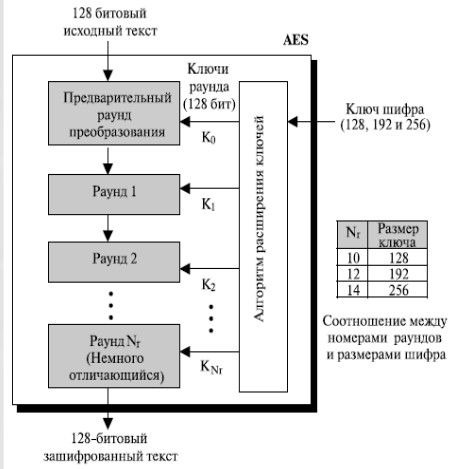
\includegraphics[width=0.7\textwidth]{img/S001.jpg}
    \caption{Структура шифра}%
\end{figure}

\FloatBarrier{}
\begin{itemize}
    \item Операции проводятся над элементами поля Галуа $GF(2^8)$.\\
    Т.е. байту соответстует многочлен $b_7 x^7 + b_6 x^6 + b_5 x^5 + b_4 x^4 + b_3 x^3 + b_2 x^2 + b_1 x + b_0$
    \item Операция умножения выполняется по модулю неприводимого многочлена $ x^8 + x^4 + x^3 + x + 1 $\\
\end{itemize}
Размер блока --- 16 байт, размер ключа --- 16, 24 или 32 байт. Размер матрицы состояний --- $4\times4$ блока

\begin{figure}[h]
    \centering
    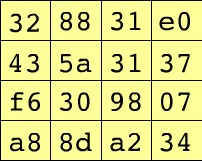
\includegraphics[width=0.3\textwidth]{img/S002.jpg}
    \caption{Матрица состояний}
\end{figure}

\begin{figure}[h]
    \centering
    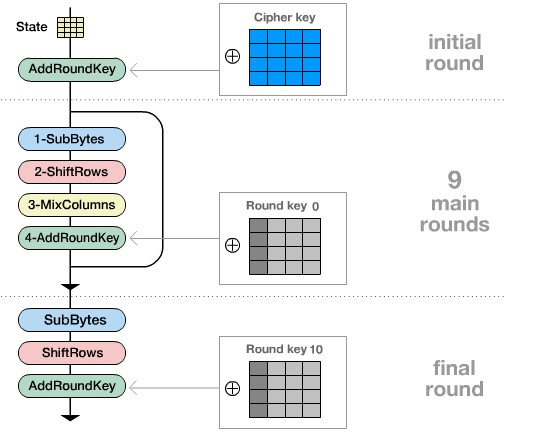
\includegraphics[width=0.8\textwidth]{img/S003.jpg}
    \caption{Операции шифра AES-192}
\end{figure}

\FloatBarrier{}
\subsection{Операции шифра}
Нижеописанные операции выполняются для всех раундов, кроме MixColumns --- она не выполняется для последнего раунда.
\subsubsection{SubBytes}
Производится нелинейная замена байтов с использованием таблицами Rijndael S-box.

\begin{figure}[h]
    \centering
    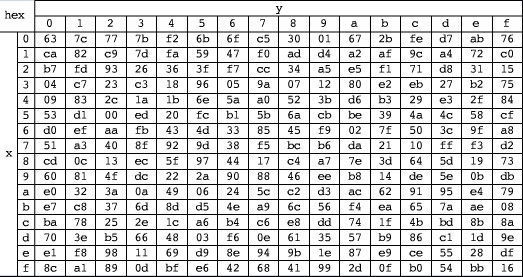
\includegraphics[width=0.9\textwidth]{img/S004.jpg}
    \caption{S-box}
\end{figure}
Первая цифра в шестнадцатеричной записи ключа --- строка, вторая --- столбец. Например, ``19'' становится ``d4''.

\FloatBarrier{}
\subsubsection{ShiftRows}
Первая строка сдвигается на 1 байт, вторая --- на 2, третья --- на 3.
\begin{figure}[h]
    \centering
    \begin{subfigure}[b]{0.3\textwidth}
    	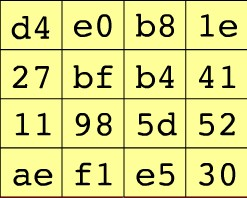
\includegraphics[width=\textwidth]{img/S006.jpg}
    	\caption{Вход ShiftRows}
    \end{subfigure}%
    \hspace{1cm}
    \begin{subfigure}[b]{0.3\textwidth}
    	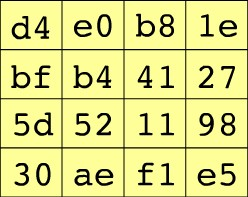
\includegraphics[width=\textwidth]{img/S007.jpg}
    	\caption{Выход ShiftRows}
    \end{subfigure}
\end{figure}

\subsubsection{MixColumns}
Каждый столбец представляется как полином третьем степени. Он умножается в $GF(2^8)$ по модулю $x^4 + 1$ на многочлен $3x^3 + x^2 + x + 2$.
\begin{figure}[h]
    \centering
    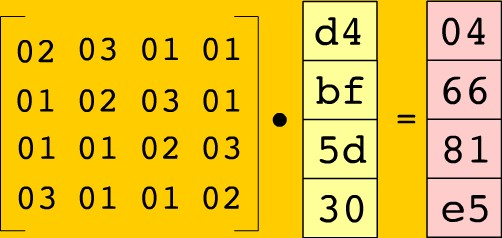
\includegraphics[width=0.4\textwidth]{img/S008.jpg}
    \caption{MixColumns}
\end{figure}

\FloatBarrier{}
\subsubsection{AddRoundKey}
Сложение каждого столбца с раундовым ключом с помощью xor.

\begin{figure}[h]
    \centering
    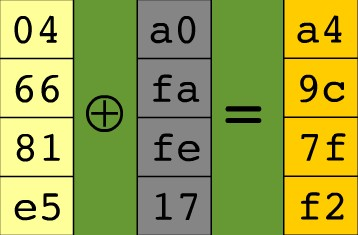
\includegraphics[width=0.3\textwidth]{img/S009.jpg}
    \caption{AddRoundKey}
\end{figure}

\FloatBarrier{}
\subsection{Генерация раундовых ключей}%
\label{subsec:theory_end}
\begin{figure}[h]
    \centering
    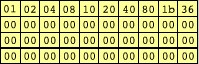
\includegraphics{img/S010.jpg}
    \caption{Rcon}
\end{figure}

\begin{enumerate}
    \item К столбцу матрицы ключа применяется побайтовый сдвиг на 1, SubBytes, его xor сложение с первым столбцом матрицы ключа и Rcon
    \begin{figure}[h]
        \centering
        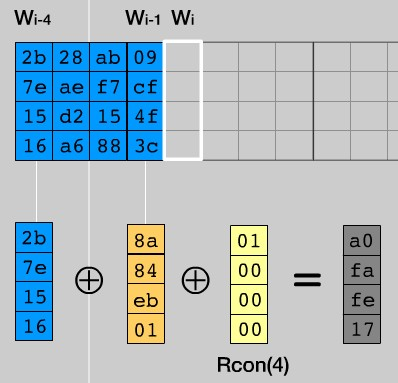
\includegraphics[width=0.5\textwidth]{img/S011.jpg}
        \caption{Первый столбец первого раундового ключа}
    \end{figure}
    \item Оставшиеся слова вычисляются xor'ом предыдущего слова со словом 4 позиции назад
    \begin{figure}[h]
        \centering
        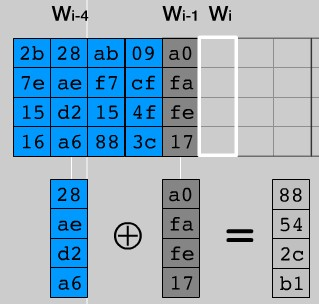
\includegraphics[width=0.5\textwidth]{img/S012.jpg}
        \caption{Второй столбец первого раундового ключа}
    \end{figure}
    \FloatBarrier{}
    \item Второй ключ вычисляется аналогичным образом по первому и т.д.
\end{enumerate}

\subsection{Ход работы}
\begin{enumerate}
    \item Изучены преобразования AES, заполнены разделы~\ref{subsec:theory_start}--\ref{subsec:theory_end}
    \item Для одного раунда преобразования выполнены вручную.\\
    Открытый текст --- \texttt{KORYTOV\_PAVELLLL}, ключ --- \texttt{6304\_VALERIEVICH} 
    \begin{enumerate}
        \item Произведено преобразование ключа и текста в шестнадцатеричный формат:
            \begin{itemize}
                \item Текст --- \texttt{4b4f5259544f565f504156454c4c4c4c}
                \item Ключ --- \texttt{363330345f56414c4552494556494348}\\
            \end{itemize}
            Получившая начальные матрицы:
            \begin{equation}
                \text{Input} = \begin{bmatrix}
                    4b  & 4f  & 52  & 59  \\
                    54  & 4f  & 56  & 5f  \\
                    50  & 41  & 56  & 45  \\
                    4c  & 4c  & 4c  & 4c  \\
                    \end{bmatrix}; \text{Key} = \begin{bmatrix}
                    36  & 33  & 30  & 34  \\
                    5f  & 56  & 41  & 4c  \\
                    45  & 52  & 49  & 45  \\
                    56  & 49  & 43  & 48  \\
                \end{bmatrix}
            \end{equation}
        \item \begin{equation}
                A_1 = AddRoundKey(\text{Input}) = \text{Input} \oplus \text{Key} = \begin{bmatrix}
                    7d & 7c & 62 & 6d \\
                    0b & 19 & 17 & 13 \\
                    15 & 13 & 1f & 00 \\
                    1a & 05 & 0f & 04 \\
                \end{bmatrix}
            \end{equation}
        \item \begin{equation}
                B_1 = SubBytes(A_1) = \begin{bmatrix}
                    ff & 10 & aa & 3c \\
                    2b & d4 & f0 & 7d \\
                    59 & 7d & c0 & 63 \\
                    a2 & 6b & 76 & f2 \\
                \end{bmatrix}
            \end{equation}
        \item \begin{equation}
                C_1 = ShiftRows(B_1) = \begin{bmatrix}
                    ff & 10 & aa & 3c \\
                    d4 & f0 & 7d & 2b \\
                    c0 & 63 & 59 & 7d \\
                    f2 & a2 & 6b & 76 \\
                \end{bmatrix}
        \end{equation}
        \item \begin{equation}
            \begin{split}
                D_1 &= MixColumns(C_1) = \\ &= \begin{bmatrix}
                    02 & 03 & 01 & 01 \\
                    01 & 02 & 03 & 01 \\
                    01 & 01 & 02 & 03 \\
                    03 & 01 & 01 & 02
                \end{bmatrix} \bullet \left( \begin{bmatrix}
                    ff \\ d4 \\ c0 \\ f2
                \end{bmatrix} , \begin{bmatrix}
                    10 \\ f0 \\ 63 \\ a2
                \end{bmatrix}, \begin{bmatrix}
                    aa \\ 7d \\ 59 \\ 6b
                \end{bmatrix} , \begin{bmatrix}
                    3c \\ 2b \\ 7d \\ 76
                \end{bmatrix} \right) = \\
                    &= \begin{bmatrix}
                        b0 & ea & fa & 0e \\
                        e5 & ec & d0 & 9b \\
                        bd & db & d8 & 77 \\
                        f1 & fc & 17 & fe
                    \end{bmatrix}
            \end{split}
        \end{equation}
        \item Раундовый ключ:
        \begin{equation}
            K_1 = \begin{bmatrix}
                1e & 2d & 1d & 29 \\
                31 & 67 & 26 & 6a \\
                17 & 45 & 0c & 49 \\
                4e & 07 & 44 & 0c
            \end{bmatrix}
        \end{equation}
        \item \begin{equation}
            \begin{split}
                A_2 &= AddRoundKey(D_1) = \\ &= \begin{bmatrix}
                        b0 & ea & fa & 0e \\
                        e5 & ec & d0 & 9b \\
                        bd & db & d8 & 77 \\
                        f1 & fc & 17 & fe
                    \end{bmatrix} \oplus \begin{bmatrix}
                1e & 2d & 1d & 29 \\
                31 & 67 & 26 & 6a \\
                17 & 45 & 0c & 49 \\
                4e & 07 & 44 & 0c
            \end{bmatrix} = \begin{bmatrix}
                ae & c7 & e7 & 27 \\
                d4 & 8b & f6 & f1 \\
                aa & 9e & d4 & 3e \\
                bf & fb & 53 & f2
            \end{bmatrix}
        \end{split}
        \end{equation}
    \end{enumerate}
    \item Проверена корректность расчётов с помощью Rijndael Inspector
    % TODO скрин
    \item Проведены наблюдения в Rijndael Flow Visualization. Результаты  на рис.~\ref{img:a:1}
    \begin{figure}[h]
        \centering
        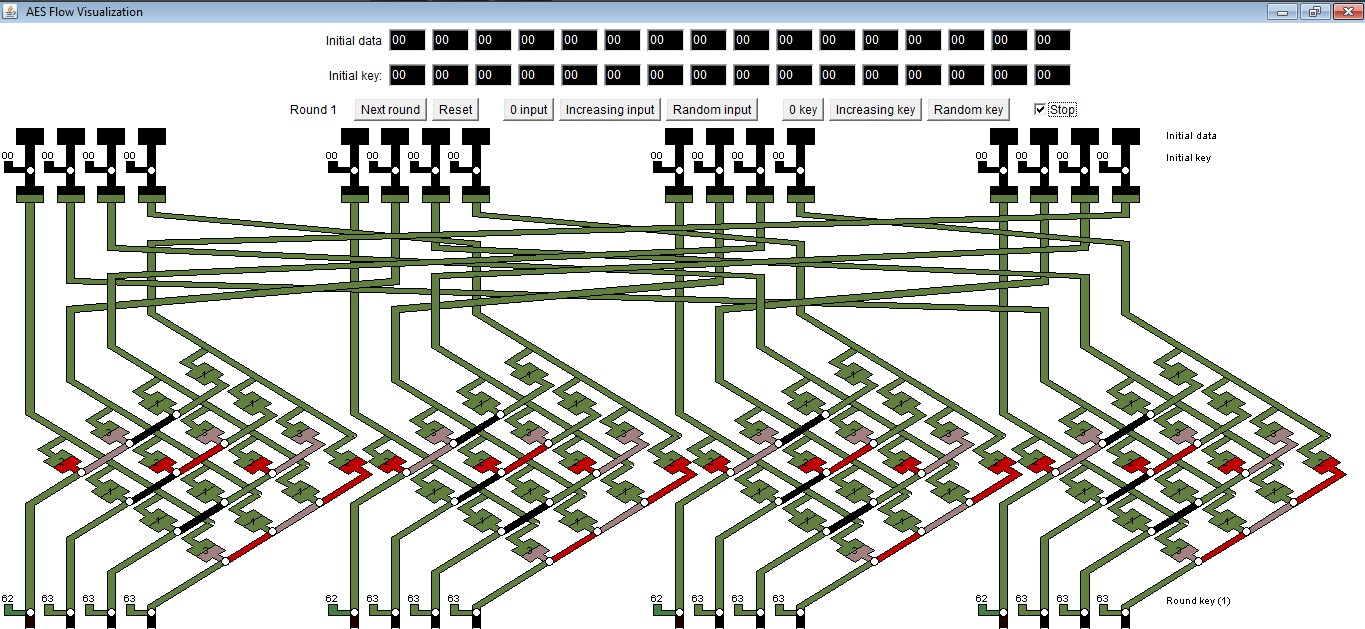
\includegraphics[width=\textheight,angle=90]{img/S013.jpg}
        \caption{Потоковая модель AES}%
        \label{img:a:1}
    \end{figure}
    
\end{enumerate}
\FloatBarrier{}
\section{Исследование финалистов конкурса AES (Rijndael, MARS, Serpent, Twofish)}
\subsection{Формулировка задания}
\begin{enumerate}
    \item Выбрать текст на английском языке (не более 120 знаков)
    \item  Создать бинарный файл с этим текстом, зашифровав и расшифровав его шифром AES на 0-м ключе
    \item  С помощью Cryptool 1 зашифровать c ключом отличным от 0 текст с использованием шифров AES, MARS, RC6, Serpent и Twofish
    \item  Приложением из Cryptool 1 вычислить энтропию исходного текста и шифротекстов, полученных в итоге. Зафиксировать результаты измерений в таблице
    \item  Приложением из Cryptool 1 оцените время проведения атаки «грубой силы» всех шифров для одного и того же шифротекста в случаях, когда известно n-2, n-4, n-6,\ldots{} 2 байт секретного ключа. Зафиксировать результаты измерений в таблице.
\end{enumerate}

\subsection{Ход работы}
\begin{enumerate}
    \item Выбран текст на английском языке: \texttt{Late in the planning of Caesar's assassination, there were two different opinions: one led by Brutus to kill only Caesar} 
    \item Создан бинарный файл
    \begin{figure}[h]
        \centering
        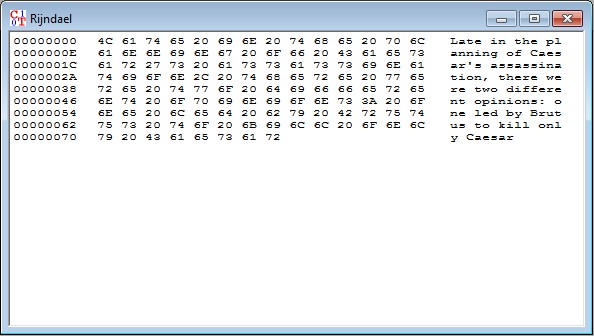
\includegraphics[width=0.7\textwidth]{img/S014.jpg}
        \caption{Бинарный файл}%
        \label{img:a:2}
    \end{figure}
    \item Произведено зашифрование файла всеми алгоритмами-финалистами коонкурса AES
    \begin{figure}[h]
        \centering
        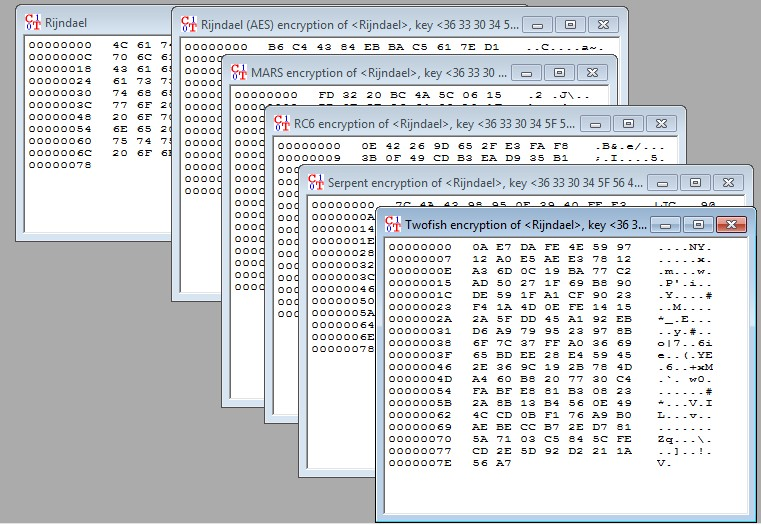
\includegraphics[width=\textwidth]{img/S015.jpg}
        \caption{Шифрование текста}%
        \label{img:}
    \end{figure}
    \FloatBarrier{}
    \item Зафиксирована энтропия исходного текста и полученных шифротекстов
    \begin{table}[h]
        \centering
        \begin{tabular}{@{}ll@{}}
            \toprule
            \textbf{Алгоритм} & \textbf{Энтропия} \\ \midrule
            Исходный текст & $4.10$ \\
            Rijndael (AES) & $6.59$ \\
            MARS & $6.50$ \\
            RC6 & $6.45$ \\
            Serpent & $6.75$ \\
            Twofish & $6.49$ \\ \bottomrule
        \end{tabular}
    \end{table}
    \item Измерено время атаки грубой силой на все шифры
    \begin{table}[h]
        \centering
        \resizebox{\textwidth}{!}{%
            \begin{tabular}{@{}llllllll@{}}
                \toprule
                \multirow{2}{*}{\textbf{Алгоритм}} & \multicolumn{7}{c}{\textbf{Известно байт}} \\
                                                   & \textit{2} & \textit{4} & \textit{6} & \textit{8} & \textit{10} & \textit{12} & \textit{14} \\ \midrule
                Rijndael (AES) & $3*10^{20}$ лет & $4*10^{15}$ лет & $7 * 10^{10}$ лет & $1 * 10^6$ лет & $16$ лет & $2$ часа & $ 1 $ сек \\
                MARS & $4*10^{20}$ лет & $6*10^{15}$ лет & $1.11 * 10^{11}$ лет & $1.6 * 10^6$ лет & $24$ года & $3$ часа & $ 1 $ сек \\
                RC6 & $3*10^{20}$ лет & $4.6*10^{15}$ лет & $7 * 10^{10}$ лет & $1.1 * 10^6$ лет & $16$ лет & $2$ часа & $ 1 $ сек \\
                Serpent & $8*10^{20}$ лет & $1.2*10^{16}$ лет & $1.9 * 10^{11}$ лет & $2.9 * 10^6$ лет & $45$ лет & $5$ часов & $ 1 $ сек \\
                Twofish & $4.8*10^{20}$ лет & $7.3*10^{15}$ лет & $1.11 * 10^{11}$ лет & $1.6 * 10^6$ лет & $26$ лет & $3$ часа & $ 1 $ сек \\ \bottomrule
            \end{tabular}%
        }
    \end{table}
    \end{enumerate}
    \FloatBarrier{}
\section{Атака \enquote{грубой силы} на AES}
\subsection{Формулировка задания}
\begin{enumerate}
    \item Найти и запустить шаблон атаки в CrypTool 2: AES Analysis using Entropy (2).
    \item  Выбрать открытый текст (примерно 1000 знаков) и загрузить его в шаблон.
    \item  Провести атаку «грубой силы» когда известно n-2, n-4, n-6 байт секретного ключа, используя в качестве оценочной функции энтропию и задействовав 1 ядро процессора. Зафиксировать затраты времени.
    \item  Выполнить атаку повторно с средним и максимальным количеством процессорных ядер. Зафиксировать затраты времени.
    \item  Сформировать текст с произвольным сообщением в формате «DEAR SIRS message THANKS» и загрузить его в шаблон. 
    \item  Провести атаку «грубой силы» когда известно n-2, n-4, n-6 байт секретного ключа, используя в качестве оценочной функции
\end{enumerate}

\subsection{Ход работы}
\begin{enumerate}
    \item Найден шаблон атаки в CrypTool 2
        \begin{figure}[h]
            \centering
            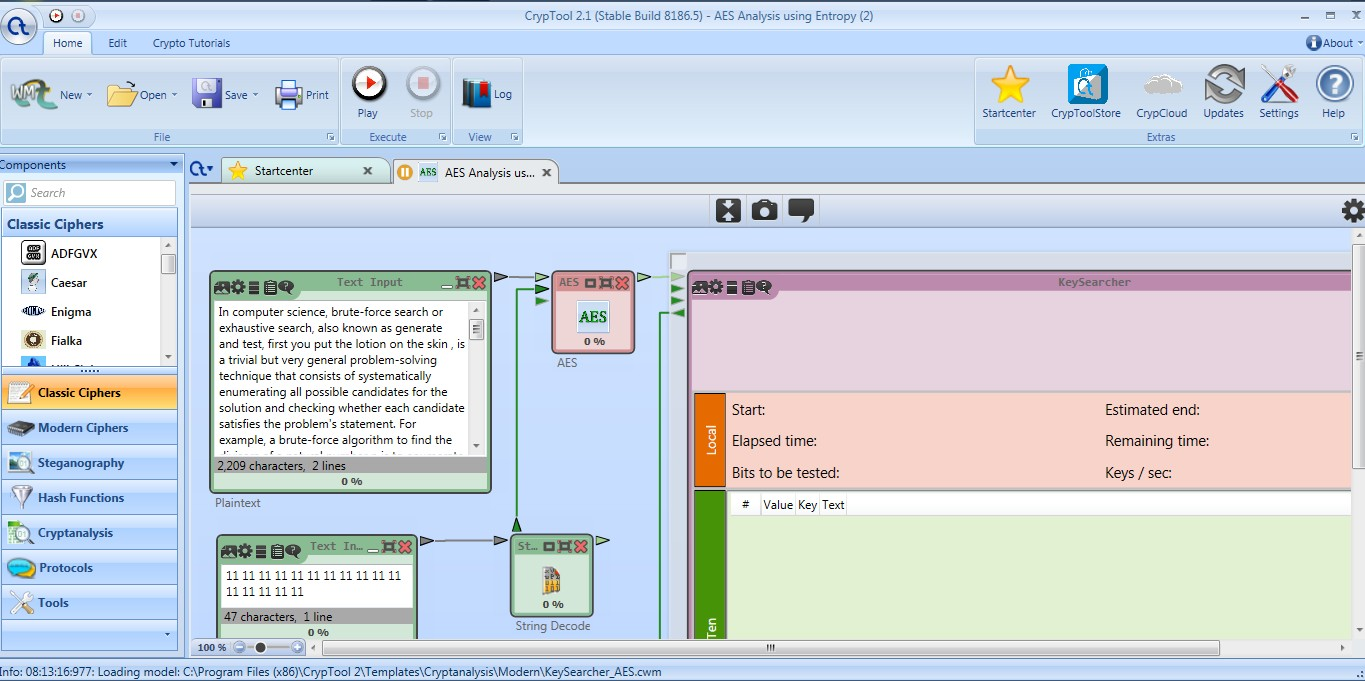
\includegraphics[width=\textwidth]{img/S016.jpg}
            \caption{Шаблон атаки в CrypTool 2}%
            \label{img:c:1}
        \end{figure}
    \item Выбран открытый текст: \texttt{The US doesn't care about Taiwan or its people. The objective is to hold Taiwan, along with South Korea and Japan and form a containment barrier that fences China in from projecting its military out into the Pacific. If China is able to break through either Taiwan or Japan, then its navy can have a shot at challenging US dominance of the blue ocean. Hence the question is how much the US is willing to sacrifice along with Japanese and maybe South Korean forces in order to contain China within the East China sea.}

        \texttt{I think all China needs to do in this situation, is build up its forces and wait. Nothing guarantees that South Korea and Japan will be on the same side in 20 years. And since China is at least ten times the size of Japan, I'm not sure Japan would be that enthusiastic about confronting them in 20 years time. That leaves the US.\@ So China's big problem would be how to discourage further US action in its ``turf'' --- i.e.\ making the costs of intervention unacceptably high.}
    \item Проведена атака на шифр с использованием разного количества ядер
        \begin{table}[h]
            \centering
            \begin{tabular}{@{}llll@{}}
                \toprule
 & \textbf{1 ядро} & \textbf{2 ядра} & \textbf{4 ядра} \\ \midrule
                14 байт & 1 сек & 1 сек & 1 сек \\
                12 байт & 1.5 часа & 47 мин & 22 мин \\
                10 байт & 10 лет & 5.5 лет & 3 года \\ \bottomrule
            \end{tabular}
        \end{table}
    \item Сформировано сообщение в указанном формате. В качестве оценочной функции использовано выражение \enquote{DEAR SIRS}. Оценка времени атаки:
        \begin{table}[h]
            \centering
            \begin{tabular}{@{}llll@{}}
                \toprule
 & \textbf{1 ядро} & \textbf{2 ядра} & \textbf{4 ядра} \\ \midrule
                14 байт & 1 сек & 1 сек & 1 сек \\
                12 байт & 21 мин & 12 мин & 7 мин \\
                10 байт & 3 года & 1.4 года & 310 дней \\ \bottomrule
            \end{tabular}
        \end{table}

\end{enumerate}

\section{Атака предссказанием дополнения на шифр AES}
\subsection{Формулировка задания}
\begin{enumerate}
    \item Найти и запустить шаблон атаки в CrypTool 2: Padding Oracle Attack on AES.\@
    \item Подготовьтесь к атаке теоретически
    \item  Внедрите во второй блок исходного текста коды символов своего имени.
    \item  Выполните 3 фазы атаки и сохраните итоговые скриншоты окончанию каждой фазы.  по окончанию каждой фазы
    \item Убедитесь, что атака удалась
\end{enumerate}

\subsection{Ход работы}
\lipsum[1] %TODO

\newpage
\section*{Выводы}
AES --- блоковый симметричный шифр, размер блока --- 128 бит. Шифр основан на подстановчно-перестановочной сети, а не на сети Фейстеля. Количество раундов:
\begin{itemize}
    \item 10 для 128-битного ключа
    \item 12 для 192-битного ключа
    \item 14 для 256-битного ключа\\
\end{itemize}

Энтропия текста и сложность атаки грубой силы сопоставима с таковой для других алгоритмов-финалистов конкурса AES, немного лучше показал себя Serpent.

Как шифрование, так и дешифрование AES распаралелливаемо. Благодаря этому атака грубой силы с использование большего количества ядер более эффективна.

Облегчить взлом может использование в качестве оценочной функции части выражения исходного текста (вместо энтропии) и знание части ключа.

Атака предсказанием дополнения в меньшей степени отражает недостатки шифра; она возможна только при его неправильном использовании.

\end{document}
